\documentclass[10pt]{article}\usepackage[margin=.65in]{geometry}\usepackage[T1]{fontenc}\usepackage{graphicx}\setlength{\parindent}{0pt}\setlength{\parskip}{7pt}\sloppy\begin{document}{\large Find visits and exact machine counter accounting}\par Producer T-1348; archive T-1350. SignedGraph::find at f123ae7053 increments operations before testing whether the vertex is a root. The counted relation retains the prior word-level Run semantics, including reading the potential after the recursive call, and adds one visit for each call.\par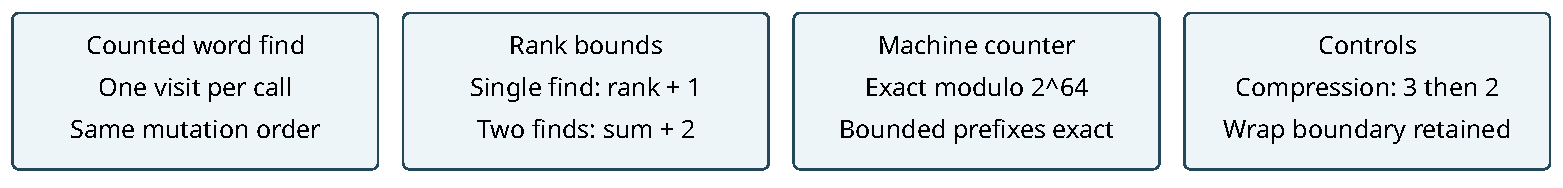
\includegraphics[width=\linewidth]{diagram.pdf}\par Result. Eleven named declarations compile. Erasing the count yields the existing Run, and every existing Run admits a counted derivation. Counts are positive. A forest-rank certificate bounds a find from x by rank(x)+1 visits. Using forest preservation between the calls, two finds have at least two visits and at most rank(u)+rank(v)+2. This is a mathematical bound in the supplied rank certificate, not a measured runtime or a tight graph-size bound.

Counter connection. Repeated UInt64 increments equal (initial counter + visits) modulo 2\textasciicircum{}64. If the initial counter plus the visit bound is below 2\textasciicircum{}64, each prefix equals the ordinary integer count. Sequential counters compose exactly; for two counted calls under the bound, the final counter is initial+a+b. The construction accounts for the source operations counter only, not field-operation counters or wall time.

Checks. Seven controls establish one root visit, three visits along a two-edge path, two visits on the same vertex after compression, an ordinary single increment, a paired increment, the last non-wrapping increment and the modular wrap boundary. Eighteen named axiom readbacks contain only propext and Quot.sound, or no axioms. Empty, renamed and sorryAx inventories are rejected. A deliberately false claim equating the wrapped word to the mathematical integer 2\textasciicircum{}64 is rejected.

Assumptions and boundary. Rank bounds use the stated forest invariant. Two-find composition also uses canonical word potentials, a positive modulus at most 2\textasciicircum{}63 and valid represented equations to apply the existing refinement and forest-preservation result. Exact machine counts require the explicit no-overflow bound. The wrap control describes Lean UInt64 modular arithmetic; it does not assert a particular Rust build's behavior beyond that bound. Stack limits, compiler refinement, other counters and allocation/partial failures remain outside this model. Independent source-fidelity review is pending.

Evidence. Each module check used one thread, 4096 MiB and a 120-second limit. Imported compiled dependencies are reused and hash-bound; no independent kernel/binary recheck occurred. Pre/post hashes do not exclude transient concurrent edits. The first counted-induction attempt and the first counter-sequence proof failed and are retained alongside the successful attempts and deliberate false theorem. The diagram describes proof components, not benchmark measurements.

Next construction. Connect cycles, negative\_cycles and zero\_coefficient increments to the source dispatcher, preserving their branch conditions and overflow bounds. Then combine counter and component-cardinality contracts with native storage representation. No scientific run, new cost ratio, cohort change or budget renewal occurred.
\end{document}